%!TEX root = ../main.tex
%%%%%%%%%%%%%%%%%%%%%%%%%%%%%%%%%%
% Links:
%
% Difficulty:
% Companies: 
%%%%%%%%%%%%%%%%%%%%%%%%%%%%%%%%%%

\chapter{Clone a linked list with random pointer}
\label{ch:clone_list_random_pointer}
\section*{Introduction}
This section discusses a very cool and interesting problem on linked list. The linked list we are dealing with here is a singly linked one, with an additional pointer that \textbf{might} point to another node in the list. The C++ definition of said list is given in Listing \ref{list:clone_list_random_pointer:list_definition}. Please note the additional field \lstinline[columns=fixed]{random} which differentiates it from other linked list definitions seen in other chapters (See Capter \ref{ch:delete_duplicates_list} and Listing \ref{list:delete_duplicates_list:linked_list}).

\begin{lstlisting}[language=c++, caption={Definition of a linked list with a random pointer.},label=list:delete_duplicates_list:linked_list]

template <class T> 
class Node
{
    public:
  T val;
  Node *next;
  Node *random;

  Node(const T &_val)
  {
    val    = _val;
    next   = nullptr;
    random = nullptr;
  }
};
\end{lstlisting}

\section{Problem statement}
\begin{exercise}
Given a linked list of the type defined in Listing \ref{list:clone_list_random_pointer:list_definition} return a deep-copy of it.
\end{exercise}

In this chapter we will be representing graphically a list using a list of pairs of integers. Each pair $(v,r)$ represent a node of the list where:
\begin{itemize}
	\item[-] $v$ is the payload of the node
	\item[-] $r$ is the index of the node that the random pointer points to. $-1$ represents \lstinline[columns=fixed]{nullptr}.
\end{itemize} 
For instance the list: $[(7,-1),(13,0),(11,4),(10,2),(1,0)]$ represent the list shown in Figure \ref{fig:clone_list_random_pointer:list1}.

\begin{figure}
	\label{fig:clone_list_random_pointer:list1}
	\centering
	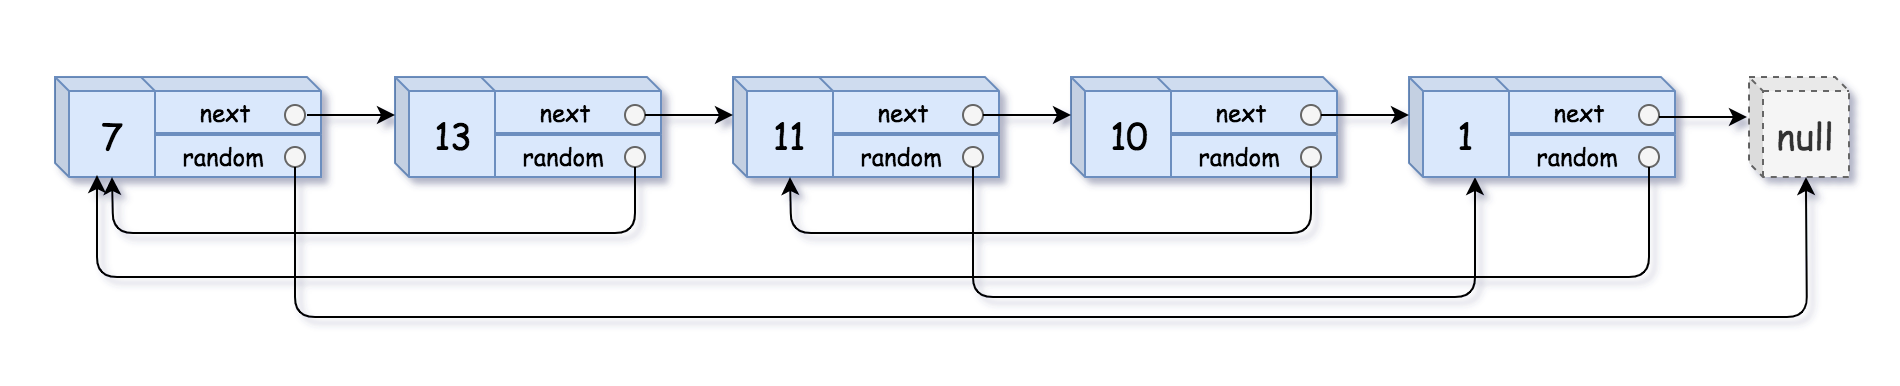
\includegraphics[scale=0.2]{sources/clone_list_random_pointer/images/random_list1}
	\caption{Linked list wit random pointer.}
\end{figure}


\section{Clarification Questions}
The problem is clearly aimed at testing the list manipulation and it is not really about algorithm design. So question related to the size of the input do not help much. Instead it is better to ask question related to the structure of the list itself to see if there is any pattern in the lists we can take advantage of.
\begin{QandA}
	\item Is it guaranteed that at least one not-null random pointer exists?
	\begin{answered}
		\textit{No, all random pointer might be null.}
	\end{answered}
	\item Can a random pointer point to itself?
	\begin{answered}
		\textit{Yes, you can have a node pointing to itself.}
	\end{answered}
	
\end{QandA}

\section{Discussion}
\label{clone_list_random_pointer:sec:discussion}
The two solutions presented in this chapter are fundamentally different and comes with asymptotic performances differences in memory.
The solution presented in Section \ref{clone_list_random_pointer:sec:bruteforce} uses additional memory (linear amount) while the second one works in constant time but it is harder to digest and to come up with in the first place.

\subsection{Linear memory solution}
\label{clone_list_random_pointer:sec:bruteforce}
The solution presented in this section can be split into a number of distinct steps:
\begin{enumerate}
	\item Create a copy of the list with all the  next and random pointers set to \lstinline[columns=fixed]{nullptr}. Save all the pointers in an \lstinline[columns=fixed]{std::vector<Node<T>*> ptrs;}.
	\item For each node in the input list, while traversing it, save in a \lstinline[columns=fixed]{map<Node<T>*, int> P} the index of that node in the list. We want to remember for each pointer the index where it appears in the original input list. 
	\item Fix the next pointers of all nodes s.t. \lstinline[columns=fixed]{ptrs[i]->next} points to  \lstinline[columns=fixed]{ptrs[i+1]}. At this point we have a new singly linked list with broken random pointers. Basically an half cloned list.
	\item At this point we can traverse the original list once again, and if the current node $c$ has a not-null random pointer $c->p$ we can query $P$ to see which index \lstinline[columns=fixed]{P[c->p]} has in the input. We know then that we need connect also the corresponding element of $c$ in the copy with the node of index \lstinline[columns=fixed]{P[c->p]} in the copy.
\end{enumerate}

The idea above can be implemented as shown in the Listing \ref{list:clone_list_random_pointer_1}


\lstinputlisting[language=c++, caption={Linear Memory solution to the problem of copying a linked list with random pointers.},label=list:clone_list_random_pointer_1]{sources/clone_list_random_pointer/clone_list_random_pointer_solution1.cpp}

